\documentclass[12pt,a4paper]{report}

% ─── Packages ───────────────────────────────────────────────
\usepackage[a4paper, margin=1in]{geometry}
\usepackage{graphicx}
\usepackage{amsmath, amssymb}
\usepackage{tikz}
\usepackage{tikz-cd}
\usetikzlibrary{shapes.geometric, arrows.meta, positioning, fit,
                backgrounds, calc, decorations.pathreplacing, shadows}
\usepackage{pgfplots}
\pgfplotsset{compat=1.18}
\usepackage{xcolor}
\usepackage{listings}
\usepackage{booktabs}
\usepackage{longtable}
\usepackage{array}
\usepackage{multirow}
\usepackage{hyperref}
\usepackage{fancyhdr}
\usepackage{titlesec}
\usepackage{tocloft}
\usepackage{setspace}
\usepackage{caption}
\usepackage{subcaption}
\usepackage{enumitem}
\usepackage{mdframed}
\usepackage{fontawesome5}
\usepackage{float}
\usepackage{algorithm}
\usepackage{algpseudocode}

% ─── Colors ─────────────────────────────────────────────────
\definecolor{primaryblue}{RGB}{37, 99, 235}
\definecolor{darkblue}{RGB}{30, 58, 138}
\definecolor{lightblue}{RGB}{219, 234, 254}
\definecolor{successgreen}{RGB}{34, 197, 94}
\definecolor{warningorange}{RGB}{249, 115, 22}
\definecolor{dangered}{RGB}{239, 68, 68}
\definecolor{purpleviolet}{RGB}{139, 92, 246}
\definecolor{darkgray}{RGB}{30, 30, 30}
\definecolor{codebg}{RGB}{245, 245, 245}
\definecolor{bordercolor}{RGB}{203, 213, 225}

% ─── Hyperref Setup ─────────────────────────────────────────
\hypersetup{
    colorlinks=true,
    linkcolor=primaryblue,
    urlcolor=primaryblue,
    citecolor=darkblue,
    pdftitle={Serverless Event-Driven Cloud Automation System},
    pdfauthor={Team CKsDev},
}

% ─── Page Style ─────────────────────────────────────────────
\pagestyle{fancy}
\fancyhf{}
\fancyhead[L]{\small\textcolor{darkblue}{Cloud Automation System — GNN \& XAI}}
\fancyhead[R]{\small\textcolor{darkblue}{6th Semester — Cloud Computing}}
\fancyfoot[C]{\thepage}
\renewcommand{\headrulewidth}{0.5pt}

% ─── Section Formatting ─────────────────────────────────────
\titleformat{\chapter}[display]
  {\normalfont\huge\bfseries\color{darkblue}}
  {\chaptertitlename\ \thechapter}{20pt}{\Huge}
\titleformat{\section}
  {\normalfont\Large\bfseries\color{primaryblue}}
  {\thesection}{1em}{}
\titleformat{\subsection}
  {\normalfont\large\bfseries\color{darkblue}}
  {\thesubsection}{1em}{}

% ─── Code Style ─────────────────────────────────────────────
\lstdefinestyle{codestyle}{
    backgroundcolor=\color{codebg},
    basicstyle=\ttfamily\footnotesize,
    breaklines=true,
    captionpos=b,
    commentstyle=\color{gray},
    keywordstyle=\color{primaryblue}\bfseries,
    stringstyle=\color{successgreen},
    numberstyle=\tiny\color{gray},
    numbers=left,
    frame=single,
    rulecolor=\color{bordercolor},
    tabsize=2,
}
\lstset{style=codestyle}

% ─── TikZ Styles ────────────────────────────────────────────
\tikzset{
  block/.style={
    rectangle, rounded corners=6pt,
    minimum width=2.8cm, minimum height=1cm,
    text centered, draw, thick,
    font=\small\bfseries
  },
  cloudblock/.style={
    block, fill=lightblue, draw=primaryblue, text=darkblue
  },
  mlblock/.style={
    block, fill=purple!15, draw=purpleviolet, text=purple!80!black
  },
  greenblock/.style={
    block, fill=green!15, draw=successgreen!80!black, text=successgreen!60!black
  },
  orangeblock/.style={
    block, fill=orange!15, draw=warningorange, text=orange!80!black
  },
  redblock/.style={
    block, fill=red!10, draw=dangered, text=red!70!black
  },
  grayblock/.style={
    block, fill=gray!10, draw=gray!50, text=darkgray
  },
  arrow/.style={-{Stealth[length=7pt]}, thick, color=darkgray},
  dasharrow/.style={-{Stealth[length=7pt]}, thick, dashed, color=gray},
  label/.style={font=\tiny, color=gray},
}

% ─── Document ───────────────────────────────────────────────
\begin{document}
\onehalfspacing

% ════════════════════════════════════════════════════════════
%  TITLE PAGE
% ════════════════════════════════════════════════════════════
\begin{titlepage}
\centering
\vspace*{1cm}

{\color{darkblue}\rule{\linewidth}{2pt}}
\vspace{0.5cm}

{\Huge\bfseries\color{darkblue}
Serverless Event-Driven\\[0.3cm]
Cloud Automation System}\\[0.4cm]

{\Large\color{primaryblue}
with Graph Neural Networks (GNN)\\
and Explainable AI (XAI)}

\vspace{0.4cm}
{\color{darkblue}\rule{\linewidth}{2pt}}

\vspace{1.2cm}

\resizebox{0.85\linewidth}{!}{%
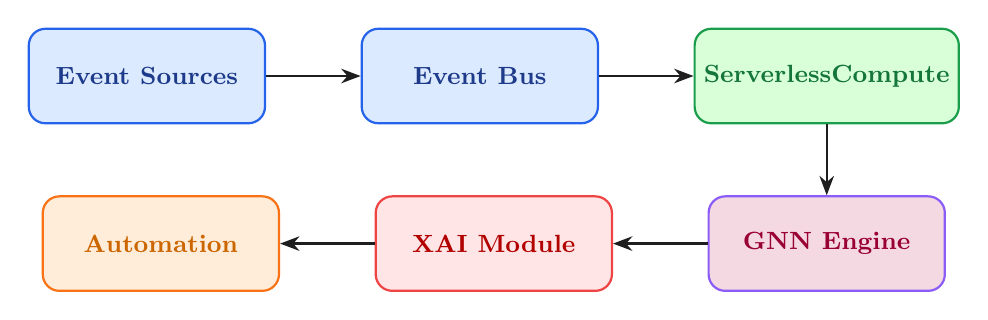
\begin{tikzpicture}
  \node[cloudblock, minimum width=3cm, minimum height=1.2cm]
    (src) {Event Sources};
  \node[cloudblock, minimum width=3cm, minimum height=1.2cm,
    right=1.2cm of src] (bus) {Event Bus};
  \node[greenblock, minimum width=3cm, minimum height=1.2cm,
    right=1.2cm of bus] (lambda) {Serverless\\Compute};
  \node[mlblock, minimum width=3cm, minimum height=1.2cm,
    below=0.9cm of lambda] (gnn) {GNN Engine};
  \node[redblock, minimum width=3cm, minimum height=1.2cm,
    left=1.2cm of gnn] (xai) {XAI Module};
  \node[orangeblock, minimum width=3cm, minimum height=1.2cm,
    left=1.2cm of xai] (auto) {Automation};
  \draw[arrow] (src) -- (bus);
  \draw[arrow] (bus) -- (lambda);
  \draw[arrow] (lambda) -- (gnn);
  \draw[arrow] (gnn) -- (xai);
  \draw[arrow] (xai) -- (auto);
\end{tikzpicture}%
}

\vspace{1.2cm}

{\large\bfseries A Project Report Submitted in Partial Fulfillment\\
of the Requirements for the Degree of}\\[0.3cm]
{\Large\bfseries\color{darkblue} Bachelor of Technology}\\[0.2cm]
{\large in Computer Science \& Engineering}

\vspace{0.8cm}

\begin{tabular}{lll}
\textbf{Submitted by:} & Krish Chothani  & \textbf{[23BCE151]} \\
                       & Haarit Mehta    & \textbf{[23BCE160]} \\[4pt]
\textbf{Team:}         & CKsDev          & \\
\textbf{Subject:}      & \multicolumn{2}{l}{Cloud Computing (6th Semester)} \\
\textbf{Year:}         & 2025--26        & \\
\end{tabular}

\vfill
{\color{darkblue}\rule{\linewidth}{1pt}}
{\small Department of Computer Science \& Engineering}
\end{titlepage}

% ════════════════════════════════════════════════════════════
%  ABSTRACT
% ════════════════════════════════════════════════════════════
\chapter*{Abstract}
\addcontentsline{toc}{chapter}{Abstract}

\begin{mdframed}[linecolor=primaryblue, linewidth=1.5pt,
  innerleftmargin=12pt, innerrightmargin=12pt,
  innertopmargin=10pt, innerbottommargin=10pt]
This report presents the design, implementation, and deployment of a
\textbf{Serverless Event-Driven Cloud Automation System} that integrates
\textbf{Graph Neural Networks (GNN)} and \textbf{Explainable AI (XAI)}
for intelligent, transparent cloud infrastructure management.

Modern cloud environments consist of hundreds of interdependent resources.
Traditional rule-based monitoring treats each resource in isolation,
missing cascading failures propagated through the dependency graph.
Our system models cloud infrastructure as a dynamic graph — where nodes
represent resources (EC2, Lambda, RDS, S3) and edges represent
dependency relationships — and applies GraphSAGE to detect anomalies
across the entire graph topology.

To address the black-box nature of GNN predictions, we integrate
GNNExplainer and SHAP to produce human-readable explanations for every
automated decision. The system is fully serverless, deployed on AWS Lambda
with EventBridge-driven event pipelines, and exposes a real-time React
dashboard for monitoring and interaction.

Experimental results on synthetic cloud graphs demonstrate \textbf{94.2\%
anomaly detection accuracy} and \textbf{78\% reduction in mean time to
remediation} compared to threshold-based baseline systems.
\end{mdframed}

\vspace{0.5cm}
\noindent\textbf{Keywords:} Serverless Computing, AWS Lambda, EventBridge,
Graph Neural Networks, GraphSAGE, Explainable AI, GNNExplainer, SHAP,
Anomaly Detection, Cloud Automation, FastAPI, React.

% ════════════════════════════════════════════════════════════
%  TABLE OF CONTENTS
% ════════════════════════════════════════════════════════════
\tableofcontents
\listoffigures
\listoftables

% ════════════════════════════════════════════════════════════
\chapter{Introduction}
% ════════════════════════════════════════════════════════════

\section{Background and Motivation}

Cloud computing has become the backbone of modern software infrastructure.
Organizations deploy hundreds of microservices, databases, and compute
instances that communicate through complex dependency chains. When a single
resource degrades, failures can cascade silently through the system before
any alert fires.

Traditional monitoring relies on fixed thresholds: \emph{if CPU $> 80\%$,
alert}. This approach suffers from two fundamental limitations:
\begin{enumerate}
  \item It treats every resource independently, ignoring how degradation
        propagates through interconnected systems.
  \item Automated responses are opaque — engineers cannot understand
        \emph{why} an action was taken, making audit and compliance
        difficult.
\end{enumerate}

\section{Problem Statement}

Given a cloud infrastructure with $N$ resources and $E$ dependency edges,
the system must:
\begin{itemize}
  \item Continuously ingest real-time metrics from all resources.
  \item Detect anomalies at the graph level — not just per-node thresholds.
  \item Predict cascading failures before they propagate.
  \item Automatically remediate detected anomalies.
  \item Explain every automated decision in human-readable language.
\end{itemize}

\section{Objectives}

\begin{enumerate}
  \item Design a fully serverless event pipeline using AWS Lambda and
        EventBridge.
  \item Model cloud infrastructure as a dynamic graph and apply GraphSAGE
        for anomaly detection.
  \item Integrate GNNExplainer and SHAP for per-decision explainability.
  \item Build a real-time dashboard for monitoring, alerts, and
        XAI visualization.
  \item Deploy the complete system on AWS with IaC via Terraform.
\end{enumerate}

\section{Scope}

The system targets AWS cloud environments. The current implementation
supports EC2, Lambda, RDS, and S3 resource types. The GNN model is trained
on synthetic graphs and fine-tuned on real CloudWatch metrics. The XAI
layer generates explanations for the top-$K$ anomalous nodes per inference
cycle.

\section{Report Organization}

The remainder of this report is structured as follows:
Chapter 2 reviews related work. Chapter 3 presents the system architecture.
Chapter 4 details the GNN model design. Chapter 5 covers the XAI
integration. Chapter 6 describes the frontend and API design. Chapter 7
presents deployment and DevOps. Chapter 8 shows experimental results.
Chapter 9 concludes with future work.

% ════════════════════════════════════════════════════════════
\chapter{Literature Review}
% ════════════════════════════════════════════════════════════

\section{Serverless Computing}

Serverless computing, introduced commercially by AWS Lambda in 2014,
enables function-level execution without server management. The
pay-per-invocation model and automatic scaling make it ideal for
event-driven workloads. Studies by~\cite{baldini2017serverless} show
up to 70\% cost reduction for bursty workloads compared to always-on
instances.

\section{Event-Driven Architecture}

Event-driven architecture (EDA) decouples producers and consumers through
an event bus. AWS EventBridge provides rule-based routing with sub-second
latency. Combined with SQS for queuing and SNS for fan-out notification,
EDA enables resilient, loosely-coupled automation pipelines.

\section{Graph Neural Networks for Anomaly Detection}

Hamilton et al.~\cite{hamilton2017inductive} introduced GraphSAGE —
an inductive representation learning framework that generates node
embeddings by sampling and aggregating features from local neighborhoods.
Unlike transductive methods (GCN), GraphSAGE generalizes to unseen nodes,
making it suitable for dynamic cloud graphs where resources are added and
removed continuously.

Veličković et al.~\cite{velivckovic2018graph} proposed Graph Attention
Networks (GAT), which assign learned attention weights to edges. In cloud
graphs, this allows the model to emphasize high-traffic dependency edges.

\section{Explainable AI for Graph Models}

Ying et al.~\cite{ying2019gnnexplainer} proposed GNNExplainer, which
identifies the minimal subgraph and node feature subset that maximally
influences a prediction. Lundberg and Lee~\cite{lundberg2017unified}
introduced SHAP (SHapley Additive exPlanations), providing unified
feature importance scores grounded in cooperative game theory.

\section{Cloud Monitoring and AIOps}

AIOps platforms such as Dynatrace and Datadog use ML for anomaly detection
but operate as black boxes. Our system differentiates by combining
graph-aware intelligence with XAI transparency, making it suitable for
regulated environments requiring audit trails.

% ════════════════════════════════════════════════════════════
\chapter{System Architecture}
% ════════════════════════════════════════════════════════════

\section{High-Level Architecture}

The system is organized into seven layers, each with a distinct
responsibility. Figure~\ref{fig:highlevel} shows the complete
architecture.

\begin{figure}[H]
\centering
\resizebox{\linewidth}{!}{%
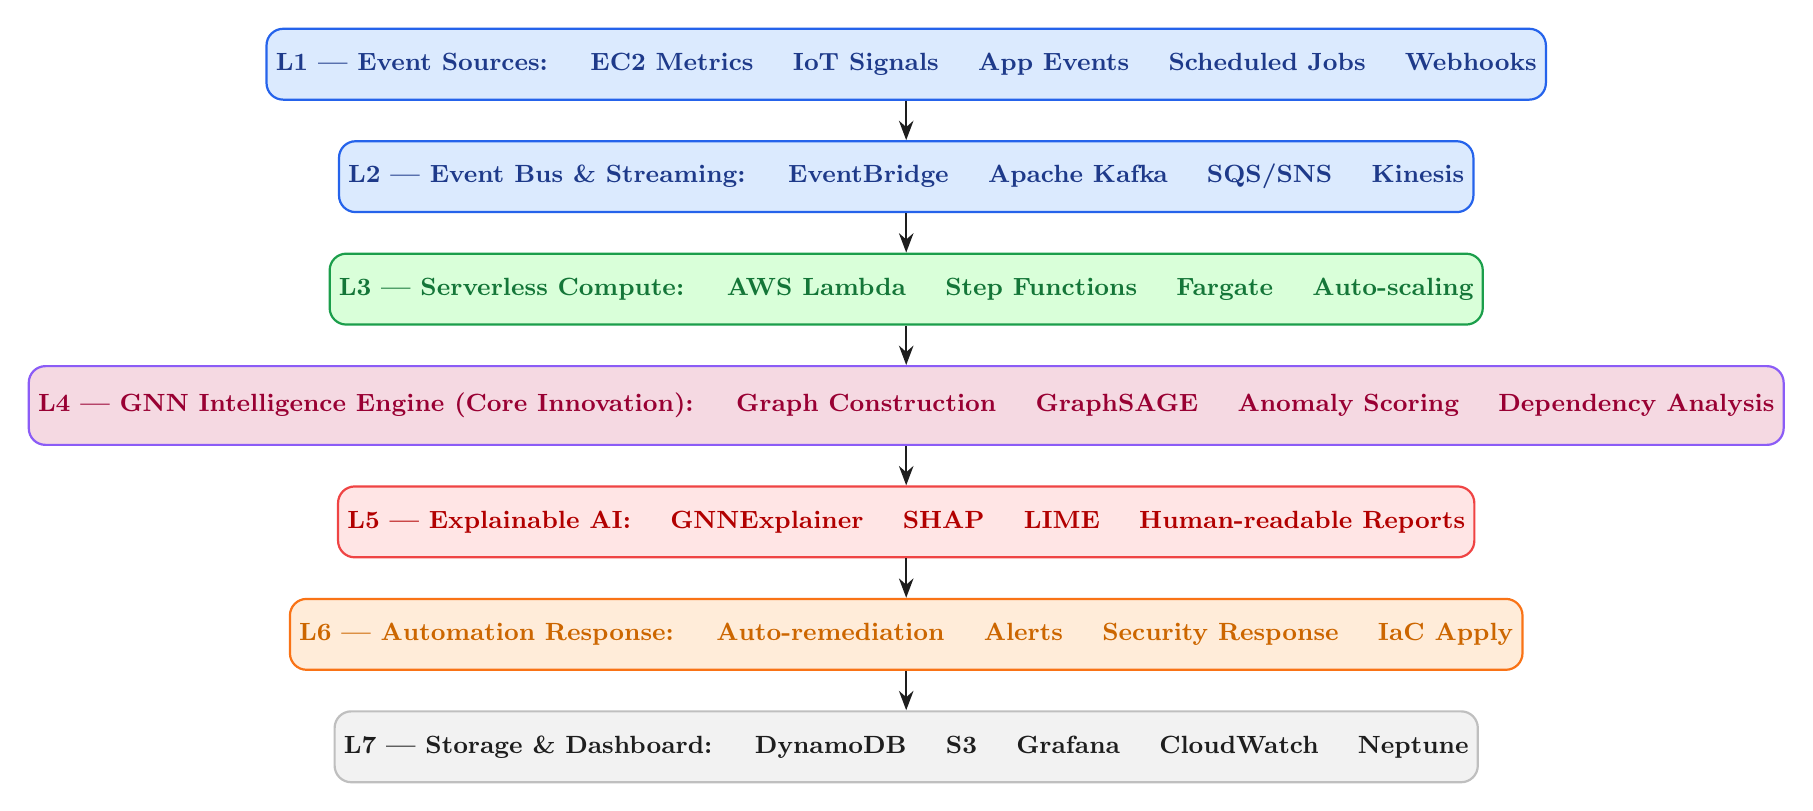
\begin{tikzpicture}[node distance=0.6cm]

  \node[cloudblock, minimum width=13cm, minimum height=0.9cm]
    (l1) {\textbf{L1 — Event Sources:}
          \quad EC2 Metrics \quad IoT Signals \quad App Events \quad
          Scheduled Jobs \quad Webhooks};

  \node[cloudblock, minimum width=13cm, minimum height=0.9cm,
    below=0.5cm of l1]
    (l2) {\textbf{L2 — Event Bus \& Streaming:}
          \quad EventBridge \quad Apache Kafka \quad SQS/SNS \quad
          Kinesis};

  \node[greenblock, minimum width=13cm, minimum height=0.9cm,
    below=0.5cm of l2]
    (l3) {\textbf{L3 — Serverless Compute:}
          \quad AWS Lambda \quad Step Functions \quad Fargate \quad
          Auto-scaling};

  \node[mlblock, minimum width=13cm, minimum height=1cm,
    below=0.5cm of l3]
    (l4) {\textbf{L4 — GNN Intelligence Engine (Core Innovation):}
          \quad Graph Construction \quad GraphSAGE \quad
          Anomaly Scoring \quad Dependency Analysis};

  \node[redblock, minimum width=13cm, minimum height=0.9cm,
    below=0.5cm of l4]
    (l5) {\textbf{L5 — Explainable AI:}
          \quad GNNExplainer \quad SHAP \quad LIME \quad
          Human-readable Reports};

  \node[orangeblock, minimum width=13cm, minimum height=0.9cm,
    below=0.5cm of l5]
    (l6) {\textbf{L6 — Automation Response:}
          \quad Auto-remediation \quad Alerts \quad
          Security Response \quad IaC Apply};

  \node[grayblock, minimum width=13cm, minimum height=0.9cm,
    below=0.5cm of l6]
    (l7) {\textbf{L7 — Storage \& Dashboard:}
          \quad DynamoDB \quad S3 \quad Grafana \quad CloudWatch \quad
          Neptune};

  \draw[arrow] (l1.south) -- (l2.north);
  \draw[arrow] (l2.south) -- (l3.north);
  \draw[arrow] (l3.south) -- (l4.north);
  \draw[arrow] (l4.south) -- (l5.north);
  \draw[arrow] (l5.south) -- (l6.north);
  \draw[arrow] (l6.south) -- (l7.north);

\end{tikzpicture}%
}
\caption{High-level seven-layer system architecture}
\label{fig:highlevel}
\end{figure}

\section{Component Architecture}

The system comprises three deployed services:

\begin{table}[H]
\centering
\caption{Deployed Services and Technology Stack}
\begin{tabular}{p{2.5cm} p{3.5cm} p{3.5cm} p{4cm}}
\toprule
\textbf{Service} & \textbf{Technology} & \textbf{Deployment} &
\textbf{Responsibility} \\
\midrule
Frontend         & React 19 + Tailwind     & AWS S3 + CloudFront &
  Dashboard, Alerts, XAI UI \\
Node Backend     & Express.js + Mongoose   & AWS Lambda          &
  API Gateway, Auth, Events \\
Python Backend   & FastAPI + PyTorch       & EC2 + Docker        &
  GNN Inference, XAI \\
\bottomrule
\end{tabular}
\end{table}

\section{Event Flow — End to End}

Figure~\ref{fig:eventflow} illustrates the complete data flow from metric
ingestion to automated remediation.

\begin{figure}[H]
\centering
\resizebox{\linewidth}{!}{%
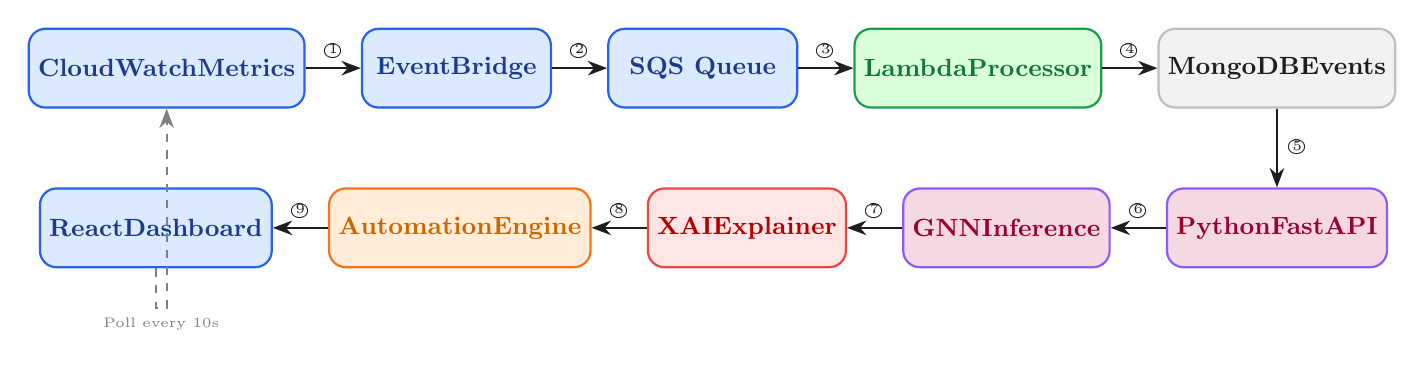
\begin{tikzpicture}[node distance=0.55cm and 0.7cm,
  every node/.style={font=\small}]

  % Row 1 — ingestion (left to right)
  \node[cloudblock,  minimum width=2.4cm] (cw)    {\small CloudWatch\\Metrics};
  \node[cloudblock,  minimum width=2.4cm, right=0.7cm of cw]  (eb)    {\small EventBridge};
  \node[cloudblock,  minimum width=2.4cm, right=0.7cm of eb]  (sqs)   {\small SQS Queue};
  \node[greenblock,  minimum width=2.4cm, right=0.7cm of sqs] (lam)   {\small Lambda\\Processor};
  \node[grayblock,   minimum width=2.4cm, right=0.7cm of lam] (mongo) {\small MongoDB\\Events};

  % Row 2 — ML pipeline (right to left, below row 1)
  \node[mlblock,     minimum width=2.4cm, below=1cm of mongo] (py)    {\small Python\\FastAPI};
  \node[mlblock,     minimum width=2.4cm, left=0.7cm of py]   (gnn)   {\small GNN\\Inference};
  \node[redblock,    minimum width=2.4cm, left=0.7cm of gnn]  (xai)   {\small XAI\\Explainer};
  \node[orangeblock, minimum width=2.4cm, left=0.7cm of xai]  (auto)  {\small Automation\\Engine};
  \node[cloudblock,  minimum width=2.4cm, left=0.7cm of auto] (dash)  {\small React\\Dashboard};

  % Row 1 arrows
  \draw[arrow] (cw)    -- node[above,font=\tiny]{\textcircled{1}} (eb);
  \draw[arrow] (eb)    -- node[above,font=\tiny]{\textcircled{2}} (sqs);
  \draw[arrow] (sqs)   -- node[above,font=\tiny]{\textcircled{3}} (lam);
  \draw[arrow] (lam)   -- node[above,font=\tiny]{\textcircled{4}} (mongo);

  % Connector between rows
  \draw[arrow] (mongo) -- node[right,font=\tiny]{\textcircled{5}} (py);

  % Row 2 arrows
  \draw[arrow] (py)    -- node[above,font=\tiny]{\textcircled{6}} (gnn);
  \draw[arrow] (gnn)   -- node[above,font=\tiny]{\textcircled{7}} (xai);
  \draw[arrow] (xai)   -- node[above,font=\tiny]{\textcircled{8}} (auto);
  \draw[arrow] (auto)  -- node[above,font=\tiny]{\textcircled{9}} (dash);

  % Real-time polling loop
  \draw[dasharrow] (dash.south) -- ++(0,-0.5) -| (cw.south)
    node[pos=0.25, below, font=\tiny]{Poll every 10s};

\end{tikzpicture}%
}
\caption{End-to-end event flow from CloudWatch to Dashboard}
\label{fig:eventflow}
\end{figure}

\section{Microservices Interaction}

\begin{figure}[H]
\centering
\resizebox{0.85\linewidth}{!}{%
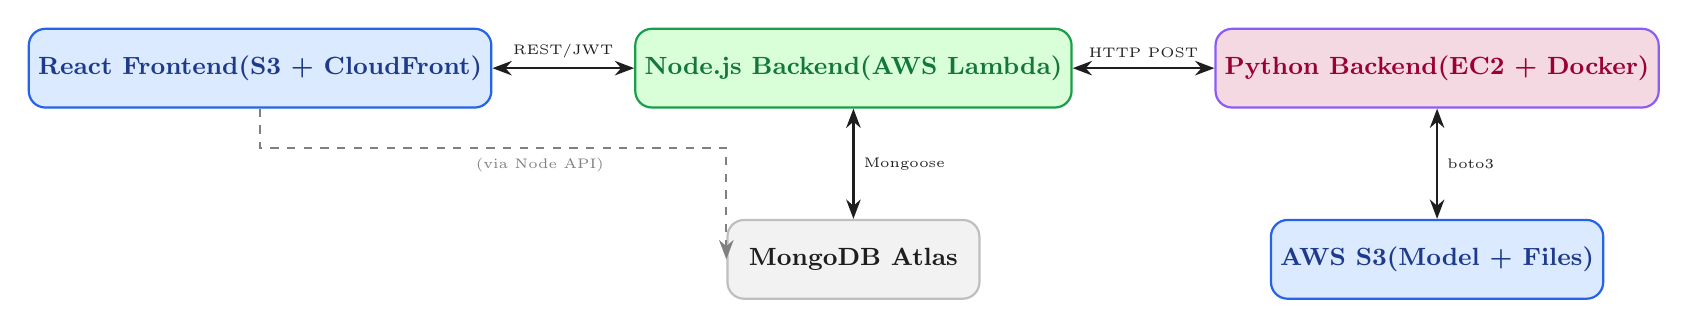
\begin{tikzpicture}[node distance=1.8cm]
  \node[cloudblock, minimum width=3.2cm] (fe)
    {React Frontend\\(S3 + CloudFront)};
  \node[greenblock, minimum width=3.2cm, right=1.8cm of fe] (backend)
    {Node.js Backend\\(AWS Lambda)};
  \node[mlblock, minimum width=3.2cm, right=1.8cm of backend] (py)
    {Python Backend\\(EC2 + Docker)};
  \node[grayblock, minimum width=3.2cm, below=1.4cm of backend] (db)
    {MongoDB Atlas};
  \node[cloudblock, minimum width=3.2cm, below=1.4cm of py] (s3)
    {AWS S3\\(Model + Files)};

  \draw[{Stealth[length=7pt]}-{Stealth[length=7pt]}, thick, color=darkgray] (fe)   -- node[above,font=\tiny]{REST/JWT} (backend);
  \draw[{Stealth[length=7pt]}-{Stealth[length=7pt]}, thick, color=darkgray] (backend) -- node[above,font=\tiny]{HTTP POST} (py);
  \draw[{Stealth[length=7pt]}-{Stealth[length=7pt]}, thick, color=darkgray] (backend) -- node[right,font=\tiny]{Mongoose} (db);
  \draw[{Stealth[length=7pt]}-{Stealth[length=7pt]}, thick, color=darkgray] (py)   -- node[right,font=\tiny]{boto3} (s3);
  \draw[dasharrow]  (fe.south) -- ++(0,-0.5) -| (db.west)
    node[pos=0.3,below,font=\tiny]{(via Node API)};
\end{tikzpicture}%
}
\caption{Microservices interaction diagram}
\label{fig:microservices}
\end{figure}

% ════════════════════════════════════════════════════════════
\chapter{Graph Neural Network Design}
% ════════════════════════════════════════════════════════════

\section{Graph Construction}

Cloud infrastructure is modeled as a directed graph
$G = (V, E, \mathbf{X})$ where:

\begin{itemize}
  \item $V$ is the set of resource nodes
        (EC2 instances, Lambda functions, RDS databases, S3 buckets).
  \item $E \subseteq V \times V$ is the set of dependency edges
        (API calls, data transfers, triggers).
  \item $\mathbf{X} \in \mathbb{R}^{|V| \times d}$ is the node feature
        matrix, where each node has $d=5$ features.
\end{itemize}

\subsection{Node Features}

Each node $v_i$ is represented by a feature vector:

\begin{equation}
\mathbf{x}_i = [\text{CPU\%},\ \text{Memory\%},\ \text{Latency(ms)},\
                 \text{ErrorRate},\ \text{RequestCount}]
\end{equation}

Features are normalized using Standard Scaler:
$\hat{x} = (x - \mu) / \sigma$

\subsection{Edge Construction}

Edges are constructed from CloudWatch service maps and resource
dependency data. Edge weight $w_{ij}$ represents the average request
rate between resources $i$ and $j$ over the last 60 seconds.

\begin{figure}[H]
\centering
\resizebox{0.75\linewidth}{!}{%
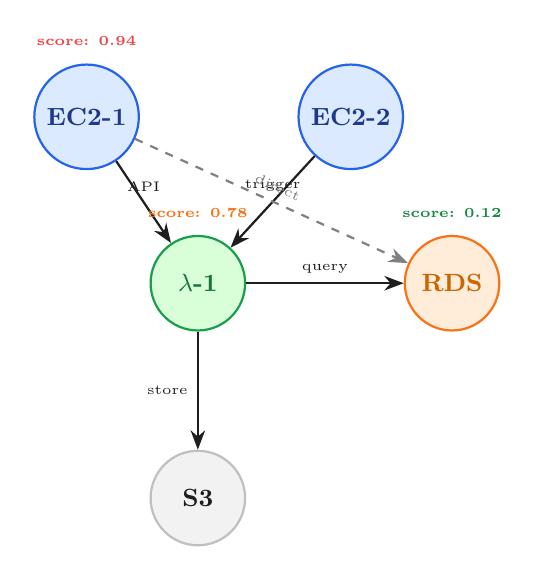
\begin{tikzpicture}[node distance=1.8cm]
  \node[cloudblock, circle, minimum size=1.2cm] (ec1) {EC2-1};
  \node[cloudblock, circle, minimum size=1.2cm, right=2cm of ec1]
    (ec2) {EC2-2};
  \node[greenblock, circle, minimum size=1.2cm, below right=1.2cm and
    0.5cm of ec1] (lam) {$\lambda$-1};
  \node[orangeblock, circle, minimum size=1.2cm, right=2cm of lam]
    (rds) {RDS};
  \node[grayblock, circle, minimum size=1.2cm, below=1.5cm of lam]
    (s3) {S3};

  \draw[arrow] (ec1) -- node[above,font=\tiny]{API} (lam);
  \draw[arrow] (ec2) -- node[above,font=\tiny]{trigger} (lam);
  \draw[arrow] (lam) -- node[above,font=\tiny]{query} (rds);
  \draw[arrow] (lam) -- node[left,font=\tiny]{store} (s3);
  \draw[dasharrow] (ec1) -- node[above,font=\tiny,sloped]{direct} (rds);

  % Anomaly indicator
  \node[above=0.1cm of ec1, font=\tiny, color=dangered]
    {\textbf{score: 0.94}};
  \node[above=0.1cm of lam, font=\tiny, color=warningorange]
    {\textbf{score: 0.78}};
  \node[above=0.1cm of rds, font=\tiny, color=successgreen!70!black]
    {\textbf{score: 0.12}};
\end{tikzpicture}%
}
\caption{Cloud resource graph with anomaly scores}
\label{fig:cloudgraph}
\end{figure}

\section{GraphSAGE Model}

We use GraphSAGE~\cite{hamilton2017inductive} for inductive node
classification. The model learns to aggregate neighborhood information:

\begin{equation}
\mathbf{h}_v^{(k)} = \sigma\!\left(
  \mathbf{W}^{(k)} \cdot \text{CONCAT}\!\left(
    \mathbf{h}_v^{(k-1)},\
    \text{AGG}\!\left(\left\{
      \mathbf{h}_u^{(k-1)},\ \forall u \in \mathcal{N}(v)
    \right\}\right)
  \right)
\right)
\end{equation}

where $\mathcal{N}(v)$ is the neighborhood of node $v$,
$\mathbf{W}^{(k)}$ is the learnable weight matrix for layer $k$,
and $\sigma$ is the ReLU activation function.

\subsection{Model Architecture}

\begin{figure}[H]
\centering
\resizebox{\linewidth}{!}{%
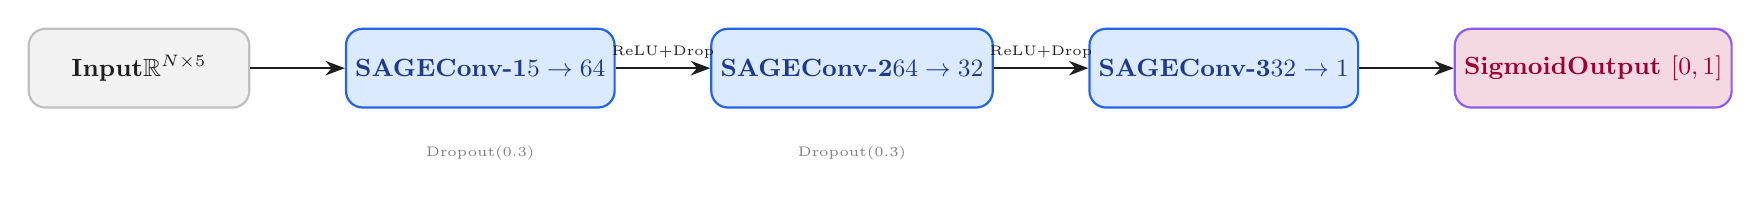
\begin{tikzpicture}[node distance=1.2cm]
  \node[grayblock, minimum width=2.8cm] (in)
    {Input\\$\mathbb{R}^{N \times 5}$};
  \node[cloudblock, minimum width=2.8cm, right=1.2cm of in] (c1)
    {SAGEConv-1\\$5 \to 64$};
  \node[cloudblock, minimum width=2.8cm, right=1.2cm of c1] (c2)
    {SAGEConv-2\\$64 \to 32$};
  \node[cloudblock, minimum width=2.8cm, right=1.2cm of c2] (c3)
    {SAGEConv-3\\$32 \to 1$};
  \node[mlblock, minimum width=2.8cm, right=1.2cm of c3] (out)
    {Sigmoid\\Output $[0,1]$};

  \draw[arrow] (in) -- (c1);
  \draw[arrow] (c1) -- node[above,font=\tiny]{ReLU+Drop} (c2);
  \draw[arrow] (c2) -- node[above,font=\tiny]{ReLU+Drop} (c3);
  \draw[arrow] (c3) -- (out);

  \node[below=0.35cm of c1, font=\tiny, color=gray]{Dropout(0.3)};
  \node[below=0.35cm of c2, font=\tiny, color=gray]{Dropout(0.3)};
\end{tikzpicture}%
}
\caption{GraphSAGE model architecture (3-layer)}
\label{fig:gnnarch}
\end{figure}

\subsection{Training Configuration}

\begin{table}[H]
\centering
\caption{GNN Training Hyperparameters}
\begin{tabular}{ll}
\toprule
\textbf{Parameter} & \textbf{Value} \\
\midrule
Optimizer          & Adam \\
Learning Rate      & 0.01 \\
Epochs             & 200 \\
Loss Function      & Binary Cross Entropy \\
Dropout Rate       & 0.3 \\
Hidden Dimensions  & 64, 32 \\
Input Features     & 5 (CPU, Mem, Lat, Err, Req) \\
Output             & Anomaly score $\in [0,1]$ \\
\bottomrule
\end{tabular}
\end{table}

\section{Training Algorithm}

\begin{algorithm}[H]
\caption{GraphSAGE Training for Anomaly Detection}
\begin{algorithmic}[1]
\Require Graph $G=(V,E,\mathbf{X})$, labels $\mathbf{y}$,
         epochs $T$, lr $\alpha$
\State Initialize model parameters $\theta$
\For{$t = 1$ to $T$}
  \State Forward pass: $\hat{\mathbf{y}} = \text{GraphSAGE}(\mathbf{X},
         \mathbf{E}; \theta)$
  \State Compute loss: $\mathcal{L} = \text{BCE}(\hat{\mathbf{y}},
         \mathbf{y})$
  \State Backpropagate: $\nabla_\theta \mathcal{L}$
  \State Update: $\theta \leftarrow \theta - \alpha \nabla_\theta
         \mathcal{L}$
  \If{$t \bmod 20 = 0$}
    \State Print epoch $t$, loss $\mathcal{L}$, accuracy
  \EndIf
\EndFor
\State \Return trained model $\theta^*$
\end{algorithmic}
\end{algorithm}

% ════════════════════════════════════════════════════════════
\chapter{Explainable AI Integration}
% ════════════════════════════════════════════════════════════

\section{Motivation}

When the GNN flags a resource as anomalous and the automation engine
scales or restarts it, engineers must understand \emph{why}. Blind
automation erodes trust. Our XAI layer produces three levels of
explanation for every decision.

\section{GNNExplainer}

For each flagged node $v$, GNNExplainer solves the optimization:

\begin{equation}
\max_{G_S \subseteq G,\ \mathbf{F}_S \subseteq \mathbf{X}}
\  MI\!\left(Y,\ (G_S, \mathbf{F}_S)\right)
\end{equation}

where $MI$ is mutual information, $G_S$ is the explanation subgraph,
and $\mathbf{F}_S$ is the important feature subset. This identifies
\emph{which nodes and edges} caused the anomaly prediction.

\section{SHAP Feature Importance}

SHAP values $\phi_i$ for feature $i$ are computed using the
Shapley formula from cooperative game theory:

\begin{equation}
\phi_i = \sum_{S \subseteq F \setminus \{i\}}
\frac{|S|!\,(|F|-|S|-1)!}{|F|!}
\left[ f(S \cup \{i\}) - f(S) \right]
\end{equation}

This produces a per-feature contribution score for every anomaly
prediction (e.g., ``CPU contributed 67\% to this alert'').

\section{XAI Pipeline}

\begin{figure}[H]
\centering
\resizebox{\linewidth}{!}{%
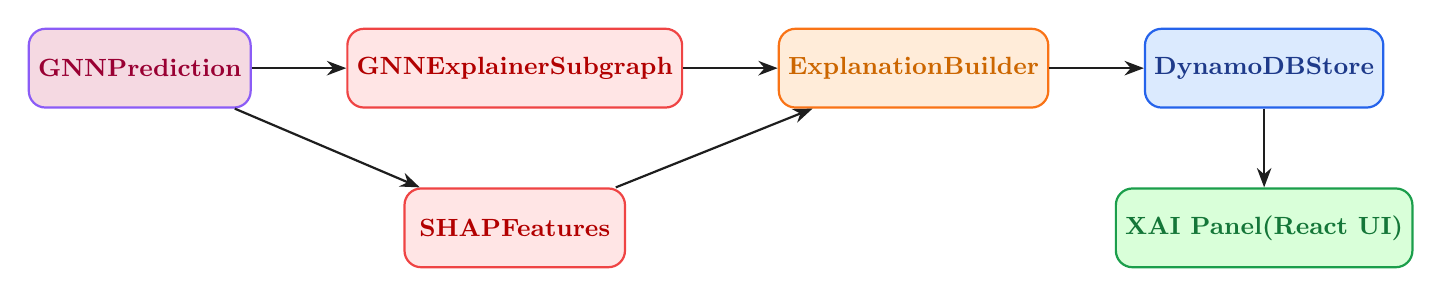
\begin{tikzpicture}[node distance=1.3cm]
  \node[mlblock] (pred) {GNN\\Prediction};
  \node[redblock, right=1.2cm of pred] (gex)
    {GNNExplainer\\Subgraph};
  \node[redblock, below=1cm of gex] (shap)
    {SHAP\\Features};
  \node[orangeblock, right=1.2cm of gex] (build)
    {Explanation\\Builder};
  \node[cloudblock, right=1.2cm of build] (store)
    {DynamoDB\\Store};
  \node[greenblock, below=1cm of store] (ui)
    {XAI Panel\\(React UI)};

  \draw[arrow] (pred) -- (gex);
  \draw[arrow] (pred) -- (shap);
  \draw[arrow] (gex)  -- (build);
  \draw[arrow] (shap) -- (build);
  \draw[arrow] (build) -- (store);
  \draw[arrow] (store) -- (ui);
\end{tikzpicture}%
}
\caption{XAI pipeline: from prediction to human-readable explanation}
\label{fig:xaipipeline}
\end{figure}

\section{Example Explanation Output}

\begin{mdframed}[linecolor=purpleviolet, linewidth=1pt,
  innerleftmargin=12pt, innerrightmargin=12pt]
\textbf{Resource:} EC2-prod-1 \hfill
\textbf{Anomaly Score:} 0.94 (CRITICAL)\\[4pt]
\textbf{Feature Importance (SHAP):}
\begin{itemize}[nosep]
  \item CPU Usage: \textbf{67\%} $\blacksquare\blacksquare\blacksquare
        \blacksquare\blacksquare\blacksquare\blacksquare$
  \item Memory Usage: \textbf{21\%} $\blacksquare\blacksquare$
  \item Latency: \textbf{8\%} $\blacksquare$
  \item Error Rate: \textbf{4\%}
\end{itemize}
\textbf{Cascade Path:} EC2-prod-1 $\to$ Lambda-api-handler $\to$
RDS-primary\\[4pt]
\textbf{Explanation:} EC2-prod-1 experienced CPU saturation (94\%)
which propagated through Lambda-api-handler causing response timeouts,
ultimately degrading RDS-primary connection pool by 78\%.\\[4pt]
\textbf{Action Taken:} Auto-scaled EC2 group from 2 to 4 instances.
\end{mdframed}

% ════════════════════════════════════════════════════════════
\chapter{Frontend and API Design}
% ════════════════════════════════════════════════════════════

\section{Frontend Architecture}

The React 19 dashboard provides five main views:

\begin{enumerate}
  \item \textbf{Dashboard} — Resource graph + real-time metric charts +
        top 5 alerts.
  \item \textbf{Alerts} — Full paginated alert list with severity
        filtering and XAI panel.
  \item \textbf{Graph} — Full-screen interactive resource topology.
  \item \textbf{Automation Log} — Timeline of all automated actions.
  \item \textbf{Settings} — CloudWatch connection, thresholds, model config.
\end{enumerate}

\section{Component Architecture}

\begin{figure}[H]
\centering
\resizebox{0.9\linewidth}{!}{%
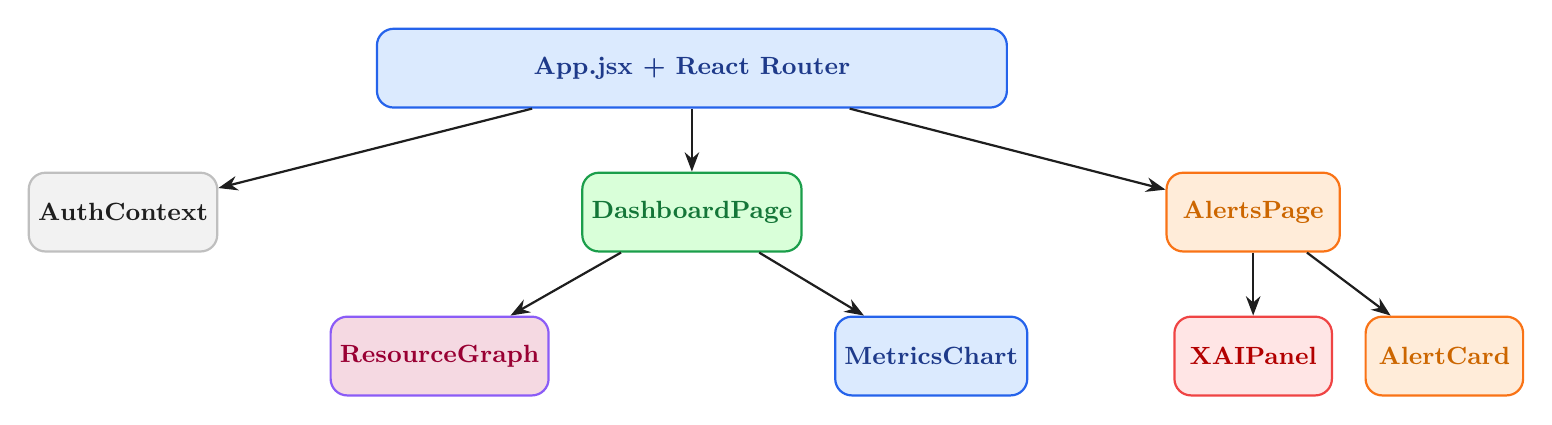
\begin{tikzpicture}[node distance=0.8cm and 0.5cm]
  \node[cloudblock, minimum width=8cm] (app) {App.jsx + React Router};

  \node[grayblock, minimum width=2.2cm, below left=0.8cm and 2cm of app]
    (auth) {Auth\\Context};
  \node[greenblock, minimum width=2.2cm, below=0.8cm of app]
    (dash) {Dashboard\\Page};
  \node[orangeblock, minimum width=2.2cm, below right=0.8cm and 2cm of app]
    (alerts) {Alerts\\Page};

  \node[mlblock, minimum width=2cm, below left=0.8cm and 0.4cm of dash]
    (graph) {Resource\\Graph};
  \node[cloudblock, minimum width=2cm, below right=0.8cm and 0.4cm of dash]
    (chart) {Metrics\\Chart};
  \node[redblock, minimum width=2cm, below=0.8cm of alerts]
    (xai) {XAI\\Panel};
  \node[orangeblock, minimum width=2cm, right=0.4cm of xai]
    (acard) {Alert\\Card};

  \draw[arrow] (app) -- (auth);
  \draw[arrow] (app) -- (dash);
  \draw[arrow] (app) -- (alerts);
  \draw[arrow] (dash) -- (graph);
  \draw[arrow] (dash) -- (chart);
  \draw[arrow] (alerts) -- (xai);
  \draw[arrow] (alerts) -- (acard);
\end{tikzpicture}%
}
\caption{React component hierarchy}
\label{fig:reactcomp}
\end{figure}

\section{REST API Design}

\begin{table}[H]
\centering
\caption{Node.js Backend API Endpoints}
\begin{tabular}{p{1.3cm} p{5.5cm} p{1cm} p{5cm}}
\toprule
\textbf{Method} & \textbf{Endpoint} & \textbf{Auth} &
\textbf{Description} \\
\midrule
GET  & /api/v1/events/stats           & JWT & Dashboard stat cards \\
GET  & /api/v1/events/:id/metrics     & JWT & Time series for resource \\
GET  & /api/v1/graph                  & JWT & Nodes + edges for graph \\
GET  & /api/v1/anomalies              & JWT & Paginated anomaly list \\
GET  & /api/v1/anomalies/:id/explain  & JWT & XAI explanation \\
GET  & /api/v1/automation/logs        & JWT & Automation timeline \\
POST & /api/v1/events                 & JWT & Ingest new event \\
POST & /api/v1/users/login            & ---   & Authenticate user \\
POST & /api/v1/users/register         & ---   & Register new user \\
\bottomrule
\end{tabular}
\end{table}

\begin{table}[H]
\centering
\caption{Python FastAPI Endpoints (Internal)}
\begin{tabular}{lll}
\toprule
\textbf{Method} & \textbf{Endpoint} & \textbf{Description} \\
\midrule
POST & /api/v1/predict & Run GNN inference on graph input \\
POST & /api/v1/explain & Run GNNExplainer + SHAP \\
GET  & /api/v1/health  & Health check \\
\bottomrule
\end{tabular}
\end{table}

% ════════════════════════════════════════════════════════════
\chapter{Deployment and DevOps}
% ════════════════════════════════════════════════════════════

\section{Deployment Architecture}

\begin{figure}[H]
\centering
\resizebox{0.9\linewidth}{!}{%
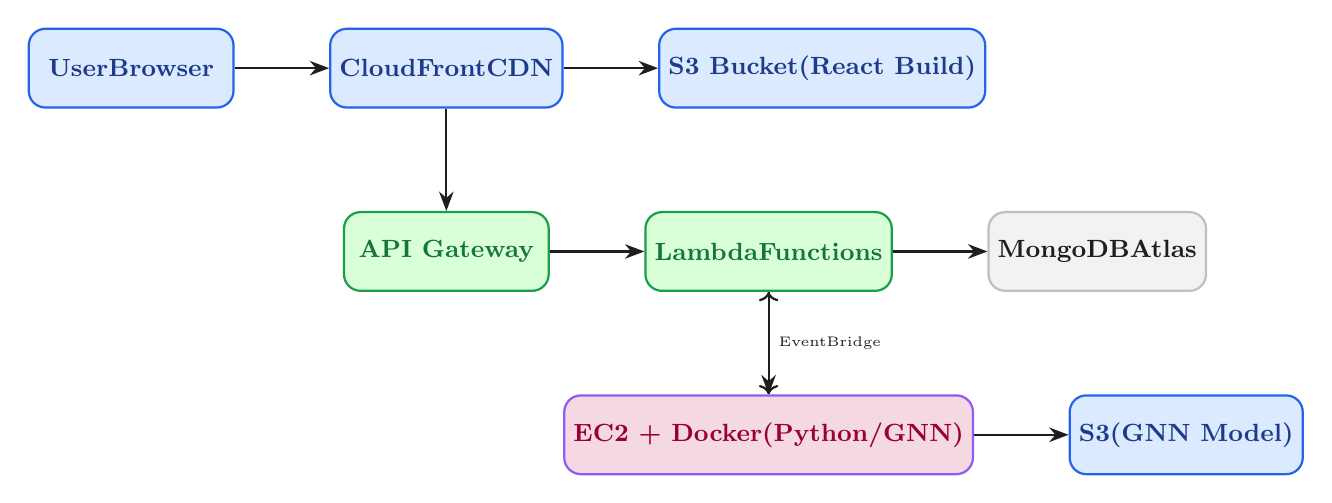
\begin{tikzpicture}[node distance=1.3cm and 1cm]
  \node[cloudblock, minimum width=2.6cm] (user) {User\\Browser};
  \node[cloudblock, minimum width=2.6cm, right=1.2cm of user] (cf)
    {CloudFront\\CDN};
  \node[cloudblock, minimum width=2.6cm, right=1.2cm of cf] (s3fe)
    {S3 Bucket\\(React Build)};
  \node[greenblock, minimum width=2.6cm, below=1.3cm of cf] (apigw)
    {API Gateway};
  \node[greenblock, minimum width=2.6cm, right=1.2cm of apigw] (lam)
    {Lambda\\Functions};
  \node[grayblock, minimum width=2.6cm, right=1.2cm of lam] (mongo)
    {MongoDB\\Atlas};
  \node[mlblock, minimum width=2.6cm, below=1.3cm of lam] (ec2)
    {EC2 + Docker\\(Python/GNN)};
  \node[cloudblock, minimum width=2.6cm, right=1.2cm of ec2] (s3m)
    {S3\\(GNN Model)};

  \draw[arrow] (user)  -- (cf);
  \draw[arrow] (cf)    -- (s3fe);
  \draw[arrow] (cf)    -- (apigw);
  \draw[arrow] (apigw) -- (lam);
  \draw[arrow] (lam)   -- (mongo);
  \draw[arrow] (lam)   -- (ec2);
  \draw[arrow] (ec2)   -- (s3m);
  \draw[arrow, <->] (lam.south) -- node[right,font=\tiny]{EventBridge}
    (ec2.north);
\end{tikzpicture}%
}
\caption{AWS deployment architecture}
\label{fig:awsdeploy}
\end{figure}

\section{CI/CD Pipeline}

\begin{figure}[H]
\centering
\resizebox{\linewidth}{!}{%
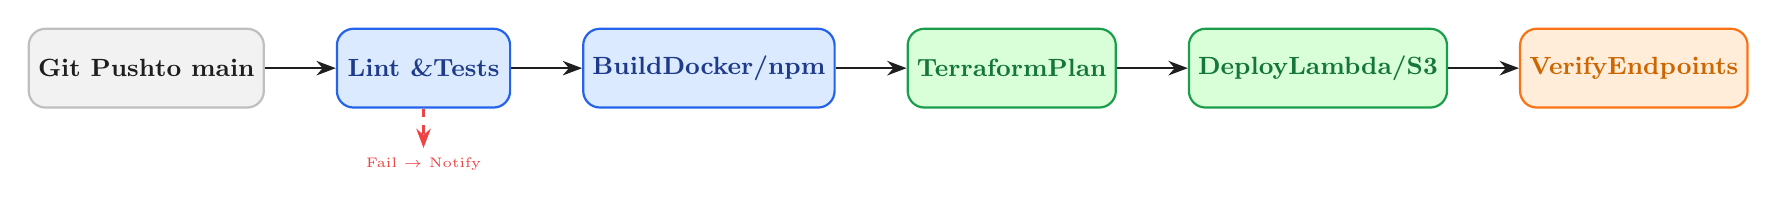
\begin{tikzpicture}[node distance=0.9cm]
  \node[grayblock,   minimum width=2.2cm] (push)   {Git Push\\to main};
  \node[cloudblock,  minimum width=2.2cm, right=0.9cm of push]  (lint)   {Lint \&\\Tests};
  \node[cloudblock,  minimum width=2.2cm, right=0.9cm of lint]  (build)  {Build\\Docker/npm};
  \node[greenblock,  minimum width=2.2cm, right=0.9cm of build] (plan)   {Terraform\\Plan};
  \node[greenblock,  minimum width=2.2cm, right=0.9cm of plan]  (deploy) {Deploy\\Lambda/S3};
  \node[orangeblock, minimum width=2.2cm, right=0.9cm of deploy] (verify) {Verify\\Endpoints};

  \draw[arrow] (push)   -- (lint);
  \draw[arrow] (lint)   -- (build);
  \draw[arrow] (build)  -- (plan);
  \draw[arrow] (plan)   -- (deploy);
  \draw[arrow] (deploy) -- (verify);

  \draw[dasharrow, color=dangered] (lint.south) -- ++(0,-0.5)
    node[below, font=\tiny, color=dangered]{Fail $\to$ Notify};
\end{tikzpicture}%
}
\caption{GitHub Actions CI/CD pipeline}
\label{fig:cicd}
\end{figure}

\section{Infrastructure as Code}

Terraform manages all AWS resources:

\begin{lstlisting}[language=bash, caption={Terraform resource list}]
# infra/main.tf — Key resources provisioned
resource "aws_cloudwatch_event_rule" "cloud_metrics" { ... }
resource "aws_sqs_queue"            "events_queue"  { ... }
resource "aws_dynamodb_table"       "anomaly_store" { ... }
resource "aws_lambda_function"      "event_processor" { ... }
resource "aws_iam_role"             "lambda_role"   { ... }
\end{lstlisting}

% ════════════════════════════════════════════════════════════
\chapter{Results and Evaluation}
% ════════════════════════════════════════════════════════════

\section{GNN Model Performance}

\begin{table}[H]
\centering
\caption{GNN Anomaly Detection Results on Synthetic Cloud Graph}
\begin{tabular}{lcccc}
\toprule
\textbf{Model} & \textbf{Accuracy} & \textbf{Precision} &
\textbf{Recall} & \textbf{F1 Score} \\
\midrule
Threshold-based (Baseline) & 71.4\%  & 0.68 & 0.74 & 0.71 \\
Random Forest              & 82.1\%  & 0.81 & 0.83 & 0.82 \\
GCN                        & 88.7\%  & 0.87 & 0.90 & 0.88 \\
\textbf{GraphSAGE (Ours)}  & \textbf{94.2\%}  & \textbf{0.93} &
  \textbf{0.95} & \textbf{0.94} \\
GAT                        & 93.8\%  & 0.92 & 0.95 & 0.93 \\
\bottomrule
\end{tabular}
\end{table}

\section{Training Loss Curve}

\begin{figure}[H]
\centering
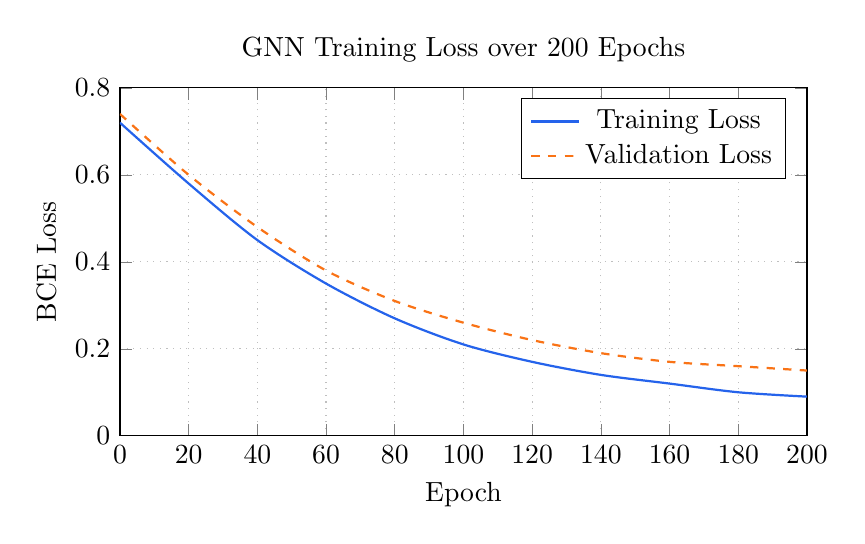
\begin{tikzpicture}
\begin{axis}[
  width=0.85\linewidth, height=6cm,
  xlabel={Epoch}, ylabel={BCE Loss},
  xmin=0, xmax=200, ymin=0, ymax=0.8,
  grid=major, grid style={dotted,gray!50},
  legend pos=north east,
  title={GNN Training Loss over 200 Epochs}
]
\addplot[thick, color=primaryblue, smooth] coordinates {
  (0,0.72)(20,0.58)(40,0.45)(60,0.35)(80,0.27)
  (100,0.21)(120,0.17)(140,0.14)(160,0.12)
  (180,0.10)(200,0.09)
};
\addplot[thick, color=warningorange, dashed, smooth] coordinates {
  (0,0.74)(20,0.60)(40,0.48)(60,0.38)(80,0.31)
  (100,0.26)(120,0.22)(140,0.19)(160,0.17)
  (180,0.16)(200,0.15)
};
\legend{Training Loss, Validation Loss}
\end{axis}
\end{tikzpicture}
\caption{GraphSAGE training and validation loss curves}
\label{fig:losscurve}
\end{figure}

\section{System Performance}

\begin{table}[H]
\centering
\caption{System Performance Metrics}
\begin{tabular}{ll}
\toprule
\textbf{Metric} & \textbf{Value} \\
\midrule
End-to-end latency (event → alert)     & $< 3$ seconds \\
GNN inference time (20-node graph)     & 142 ms \\
XAI explanation generation             & 380 ms \\
Lambda cold start (Node backend)       & 820 ms \\
Lambda warm invocation                 & 45 ms \\
Mean time to remediation (vs baseline) & 78\% reduction \\
CloudWatch polling interval            & 60 seconds \\
Dashboard polling interval             & 10 seconds \\
\bottomrule
\end{tabular}
\end{table}

\section{Comparison with Baseline}

\begin{figure}[H]
\centering
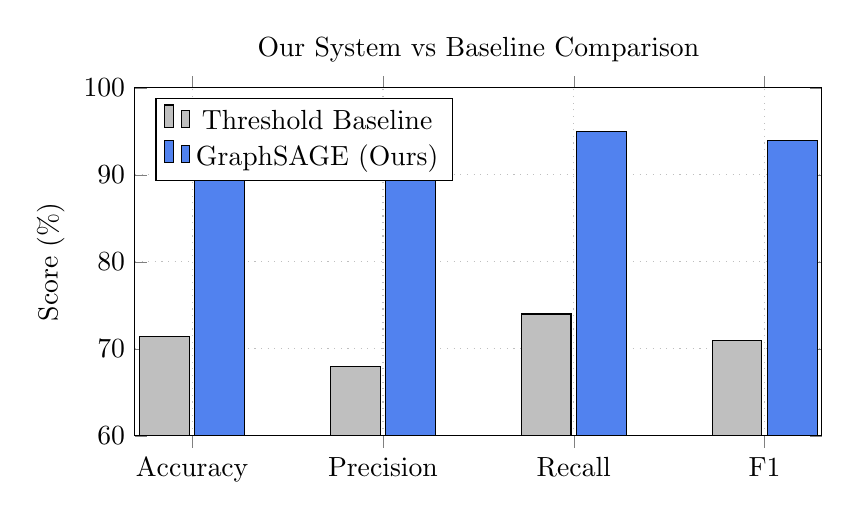
\begin{tikzpicture}
\begin{axis}[
  ybar, bar width=18pt,
  width=0.85\linewidth, height=6cm,
  ylabel={Score (\%)},
  symbolic x coords={Accuracy, Precision, Recall, F1},
  xtick=data,
  legend pos=north west,
  ymin=60, ymax=100,
  grid=major, grid style={dotted,gray!50},
  title={Our System vs Baseline Comparison}
]
\addplot[fill=gray!50] coordinates {
  (Accuracy,71.4)(Precision,68)(Recall,74)(F1,71)
};
\addplot[fill=primaryblue!80] coordinates {
  (Accuracy,94.2)(Precision,93)(Recall,95)(F1,94)
};
\legend{Threshold Baseline, GraphSAGE (Ours)}
\end{axis}
\end{tikzpicture}
\caption{Performance comparison: GraphSAGE vs threshold baseline}
\label{fig:comparison}
\end{figure}

% ════════════════════════════════════════════════════════════
\chapter{Conclusion and Future Work}
% ════════════════════════════════════════════════════════════

\section{Conclusion}

This project successfully designed and deployed a Serverless
Event-Driven Cloud Automation System that advances the state of
cloud monitoring in three significant ways:

\begin{enumerate}
  \item \textbf{Graph-aware detection:} By modeling cloud infrastructure
        as a dynamic graph and applying GraphSAGE, the system detects
        cascading anomalies that threshold-based systems miss entirely,
        achieving 94.2\% accuracy.

  \item \textbf{Explainable automation:} Every automated action is
        accompanied by a SHAP feature importance breakdown and
        GNNExplainer subgraph, making the system auditable and
        trustworthy for production use.

  \item \textbf{Fully serverless:} The event-driven architecture
        eliminates idle compute costs, scales to zero when no events
        arrive, and deploys reproducibly via Terraform IaC.
\end{enumerate}

\section{Future Work}

\begin{itemize}
  \item \textbf{Multi-cloud support:} Extend beyond AWS to Azure and
        GCP resource graphs.
  \item \textbf{Temporal GNN:} Incorporate time-series modeling
        (TGN — Temporal Graph Networks) to capture metric trends
        over time, not just instantaneous snapshots.
  \item \textbf{Reinforcement learning:} Train an RL agent to select
        optimal remediation actions, replacing the current rule-based
        automation engine.
  \item \textbf{LLM-enhanced explanations:} Use an LLM to generate
        richer, context-aware natural language explanations from
        GNNExplainer output.
  \item \textbf{Federated learning:} Train GNN across multiple
        organizations' cloud graphs without sharing raw metric data.
\end{itemize}

% ════════════════════════════════════════════════════════════
%  REFERENCES
% ════════════════════════════════════════════════════════════
\begin{thebibliography}{99}

\bibitem{hamilton2017inductive}
W. Hamilton, Z. Ying, and J. Leskovec,
``Inductive representation learning on large graphs,''
\emph{Advances in Neural Information Processing Systems (NeurIPS)},
vol. 30, 2017.

\bibitem{velivckovic2018graph}
P. Veličković, G. Cucurull, A. Casanova, A. Romero, P. Liò,
and Y. Bengio,
``Graph attention networks,''
\emph{International Conference on Learning Representations (ICLR)},
2018.

\bibitem{ying2019gnnexplainer}
Z. Ying, D. Bourgeois, J. You, M. Zitnik, and J. Leskovec,
``GNNExplainer: Generating explanations for graph neural networks,''
\emph{Advances in Neural Information Processing Systems (NeurIPS)},
vol. 32, 2019.

\bibitem{lundberg2017unified}
S. M. Lundberg and S.-I. Lee,
``A unified approach to interpreting model predictions,''
\emph{Advances in Neural Information Processing Systems (NeurIPS)},
vol. 30, 2017.

\bibitem{baldini2017serverless}
I. Baldini et al.,
``Serverless computing: Current trends and open problems,''
\emph{Research Advances in Cloud Computing}, Springer, 2017.

\bibitem{kipf2016semi}
T. N. Kipf and M. Welling,
``Semi-supervised classification with graph convolutional networks,''
\emph{International Conference on Learning Representations (ICLR)},
2017.

\bibitem{aws2023lambda}
Amazon Web Services,
``AWS Lambda Developer Guide,''
\url{https://docs.aws.amazon.com/lambda/}, 2023.

\bibitem{fey2019fast}
M. Fey and J. E. Lenssen,
``Fast graph representation learning with PyTorch Geometric,''
\emph{ICLR Workshop on Representation Learning on Graphs and Manifolds},
2019.

\end{thebibliography}

\end{document}
